% !TeX root = OptCuts.tex

\section{Evaluation}
\label{sec:results}

We tested our approach on a benchmark containing a diverse set of 70 surfaces commonly used in geometry processing research.  The meshes from this benchmark  are organic shapes with intricate geometric details composed of XXX to YYY \vova{add numbers} vertices, and are topological disks or spheres \vova{add higher genus if we have it}. In addition, we stress-test the scalability of various methods on a Lucy model that has 48k vertices at the highest resolution. 

Our method always achieves the desired distortion bound $b_d$ which is defined by symmetric Dirichlet energy, and we use our normalized seam length $E_{s}$ as an evaluation metric (where the goal is to achieve the desired distortion with minimal seams). Since $E_{s}$ is normalized by square root of mesh area it provides a comparable measure across all examples and methods. 

We implemented our framework in libigl~\cite{libigl} library\footnote{~We also plan to make our implementation publicly available.}. All experiments presented in this paper were executed on a Macbook Pro with 3.1 GHz quad-core Intel Core i7 CPU and 16 GB 2133 MHz LPDDR3 memory.

%We implement our methods based on libigl\ \cite{libigl} and test it on a Macbook Pro with 3.1 GHz quad-core Intel Core i7 CPU and 16 GB 2133 MHz LPDDR3 memory.
% @misc{libigl,
%   title = {{libigl}: A simple {C++} geometry processing library},
%   author = {Alec Jacobson and Daniele Panozzo and others},
%   note = {http://libigl.github.io/libigl/},
%   year = {2017},
% }


\subsection{Method Evaluation}
\minchen{Add energy plot to show convergence?}

%We directly use our normalized seam length $E_{s}$ as the evaluation metric as it is both shape aware and mesh independent. For comparisons, we always generate UV maps under the same distortion bound either set equally or obtained from the output that are compared with.
%Moreover, this metric also fits in well with practical scenarios where the control of distortions are more intuitive to the users and as-short-as-possible seams are expected.

We execute our method on the benchmark using various target distortion bounds of $b_d \in \{4.2, 4.1, 4.05\}$, and also disabling and enabling global bijectivity constraints. 
In all cases our fully automatic method produces output that satisfies the desired constraints and introduces reasonably few seams (Figures~\ref{fig:our_impressive_results}). We observe that more constraints such as tighter distortion bound or global bijectivity necessitate longer seams (Figure~\ref{fig:ours_various_bounds}) and increase computational cost (Table~\ref{tb:stats_OptCuts}).

%We evaluate our method with/without global bijectivity by running them on 70 input surfaces including both disk-topology and closed surfaces (some are with \minchen{[TODO] high genus}), setting $b_d$ to $4.2$, $4.1$, and $4.05$ (Table~\ref{tb:stats_OptCuts}). Our methods automatically generate high quality UV maps given any distortion bounds for all inputs without any user assistance ().

\begin{figure}[t]
\centering
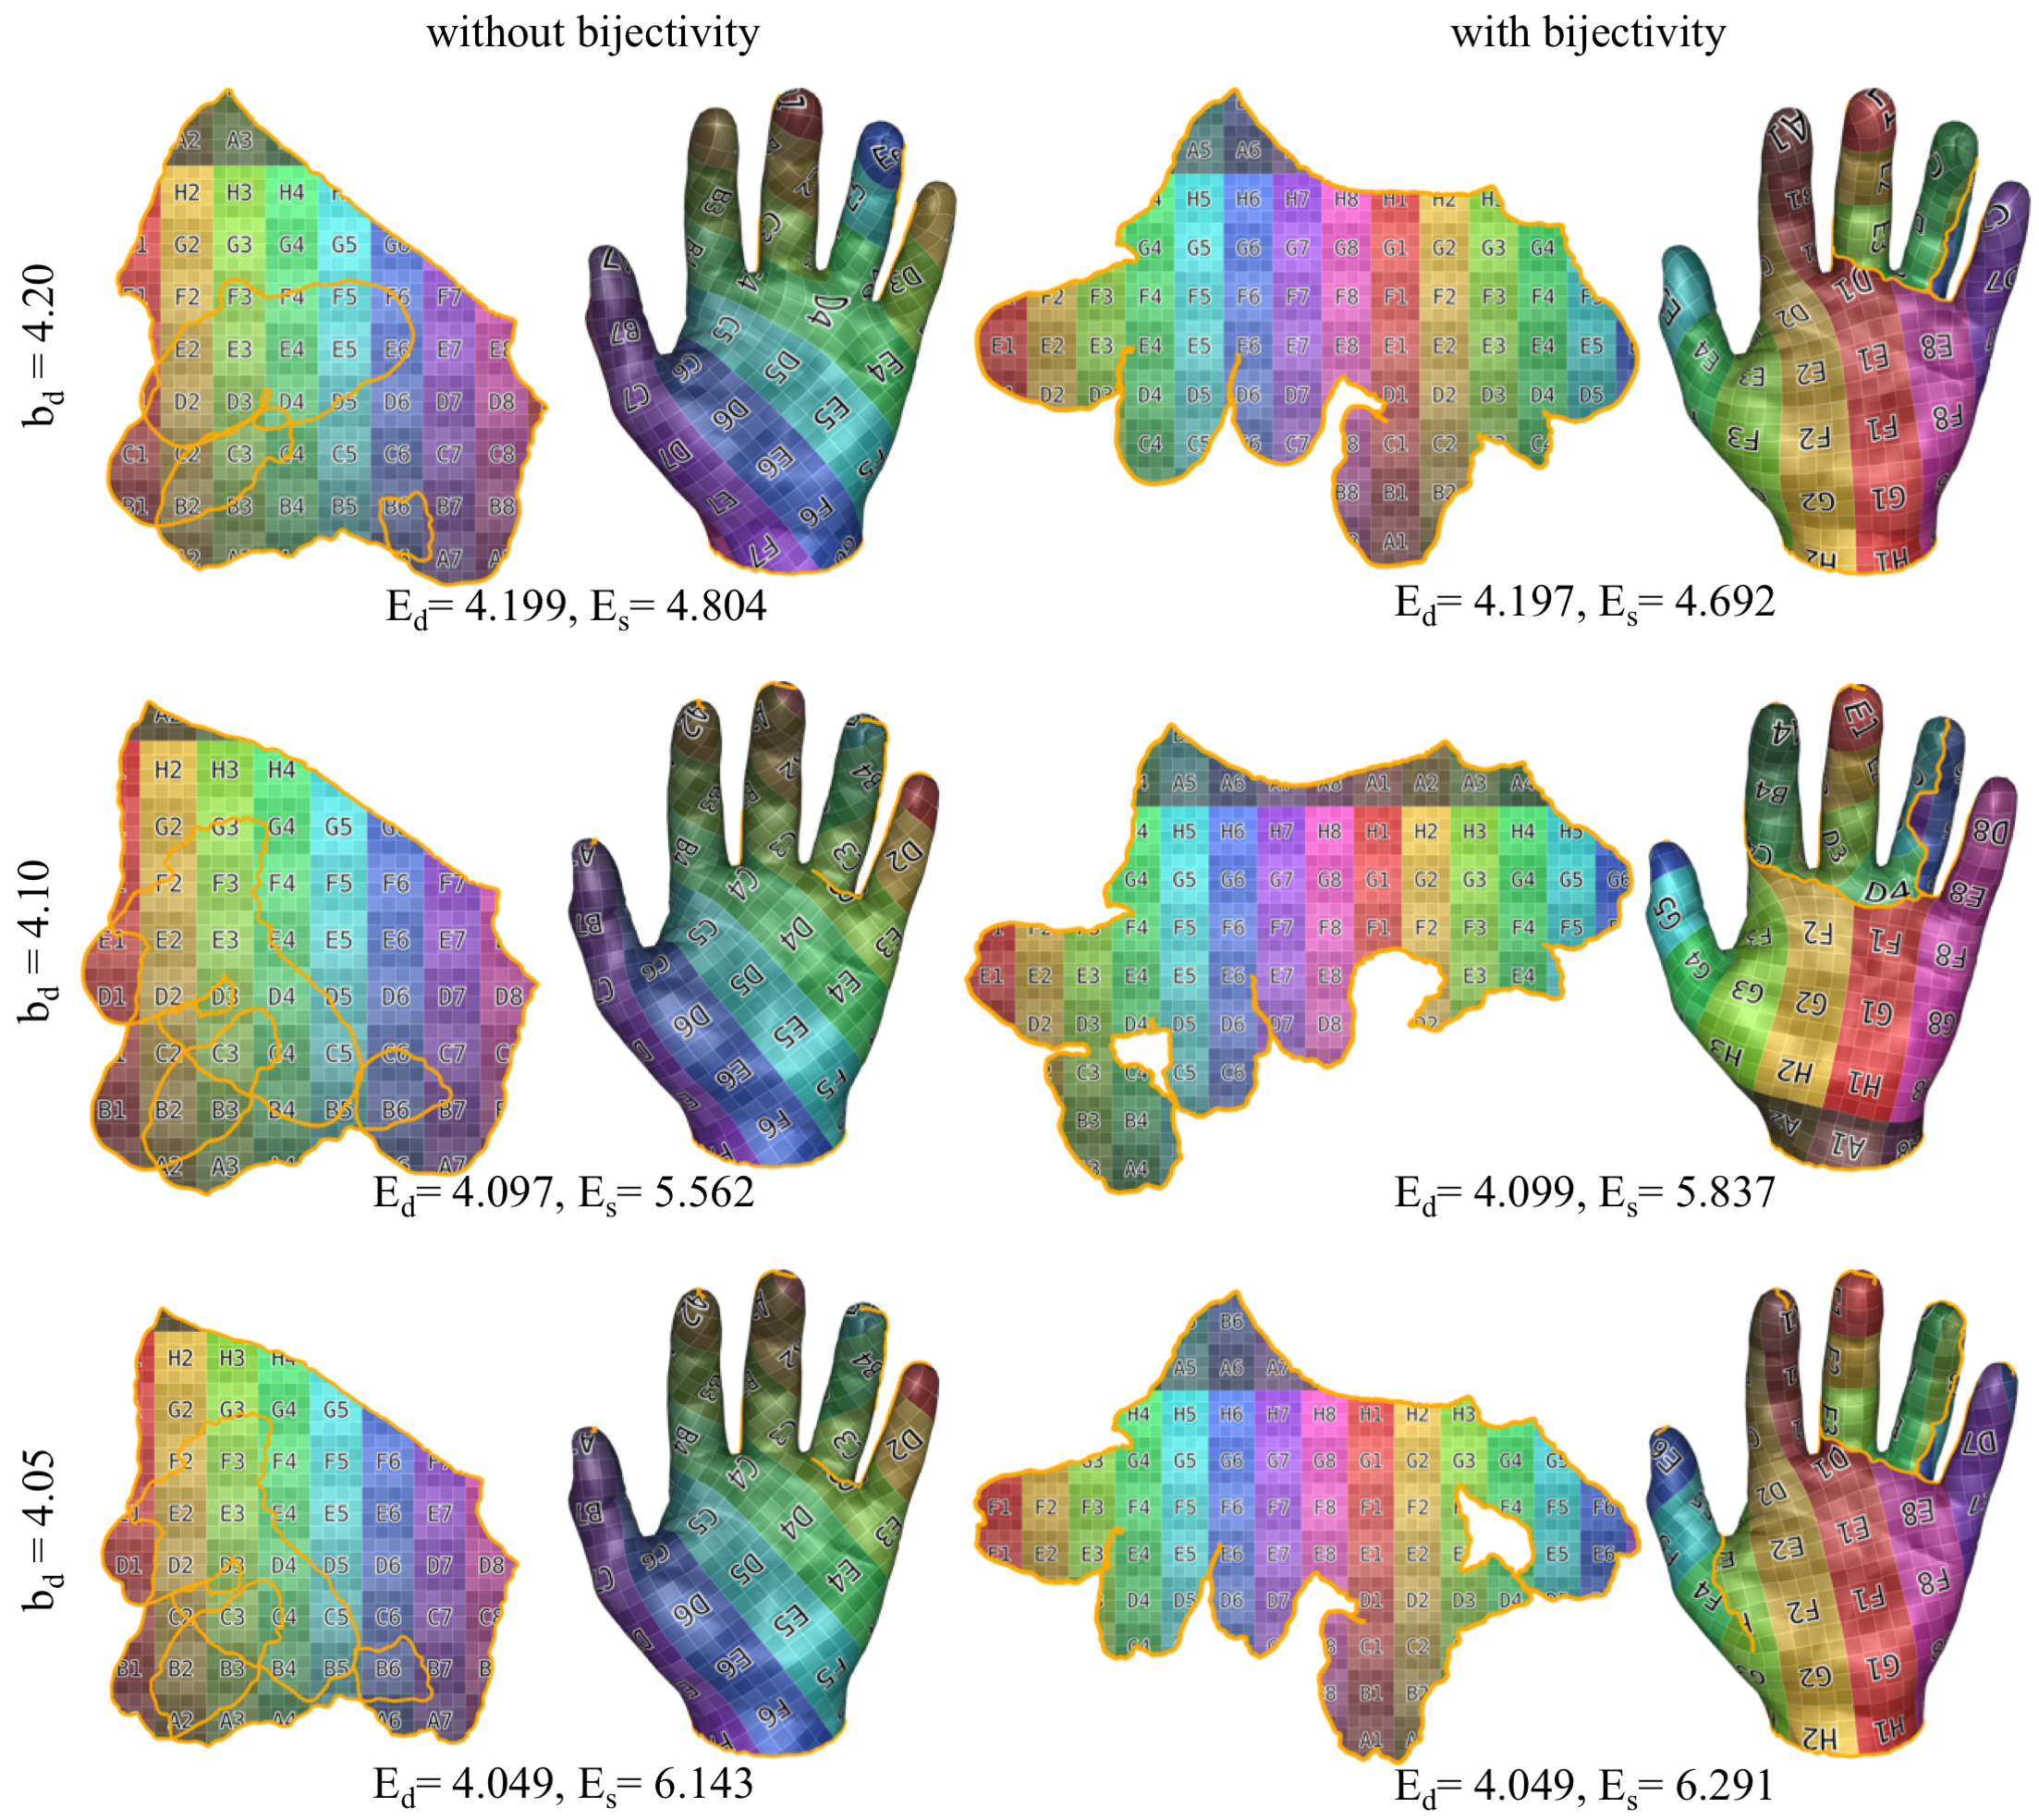
\includegraphics[width=\linewidth]{fig/our_impressive_results_left.png}
\caption{UV maps generated for a hand model by OptCuts with/without bijectivity with $b_d$ set to $4.2$, $4.1$, and $4.05$ from top to bottom.}
\label{fig:ours_various_bounds}
\end{figure}
%
\begin{figure}[t]
\centering
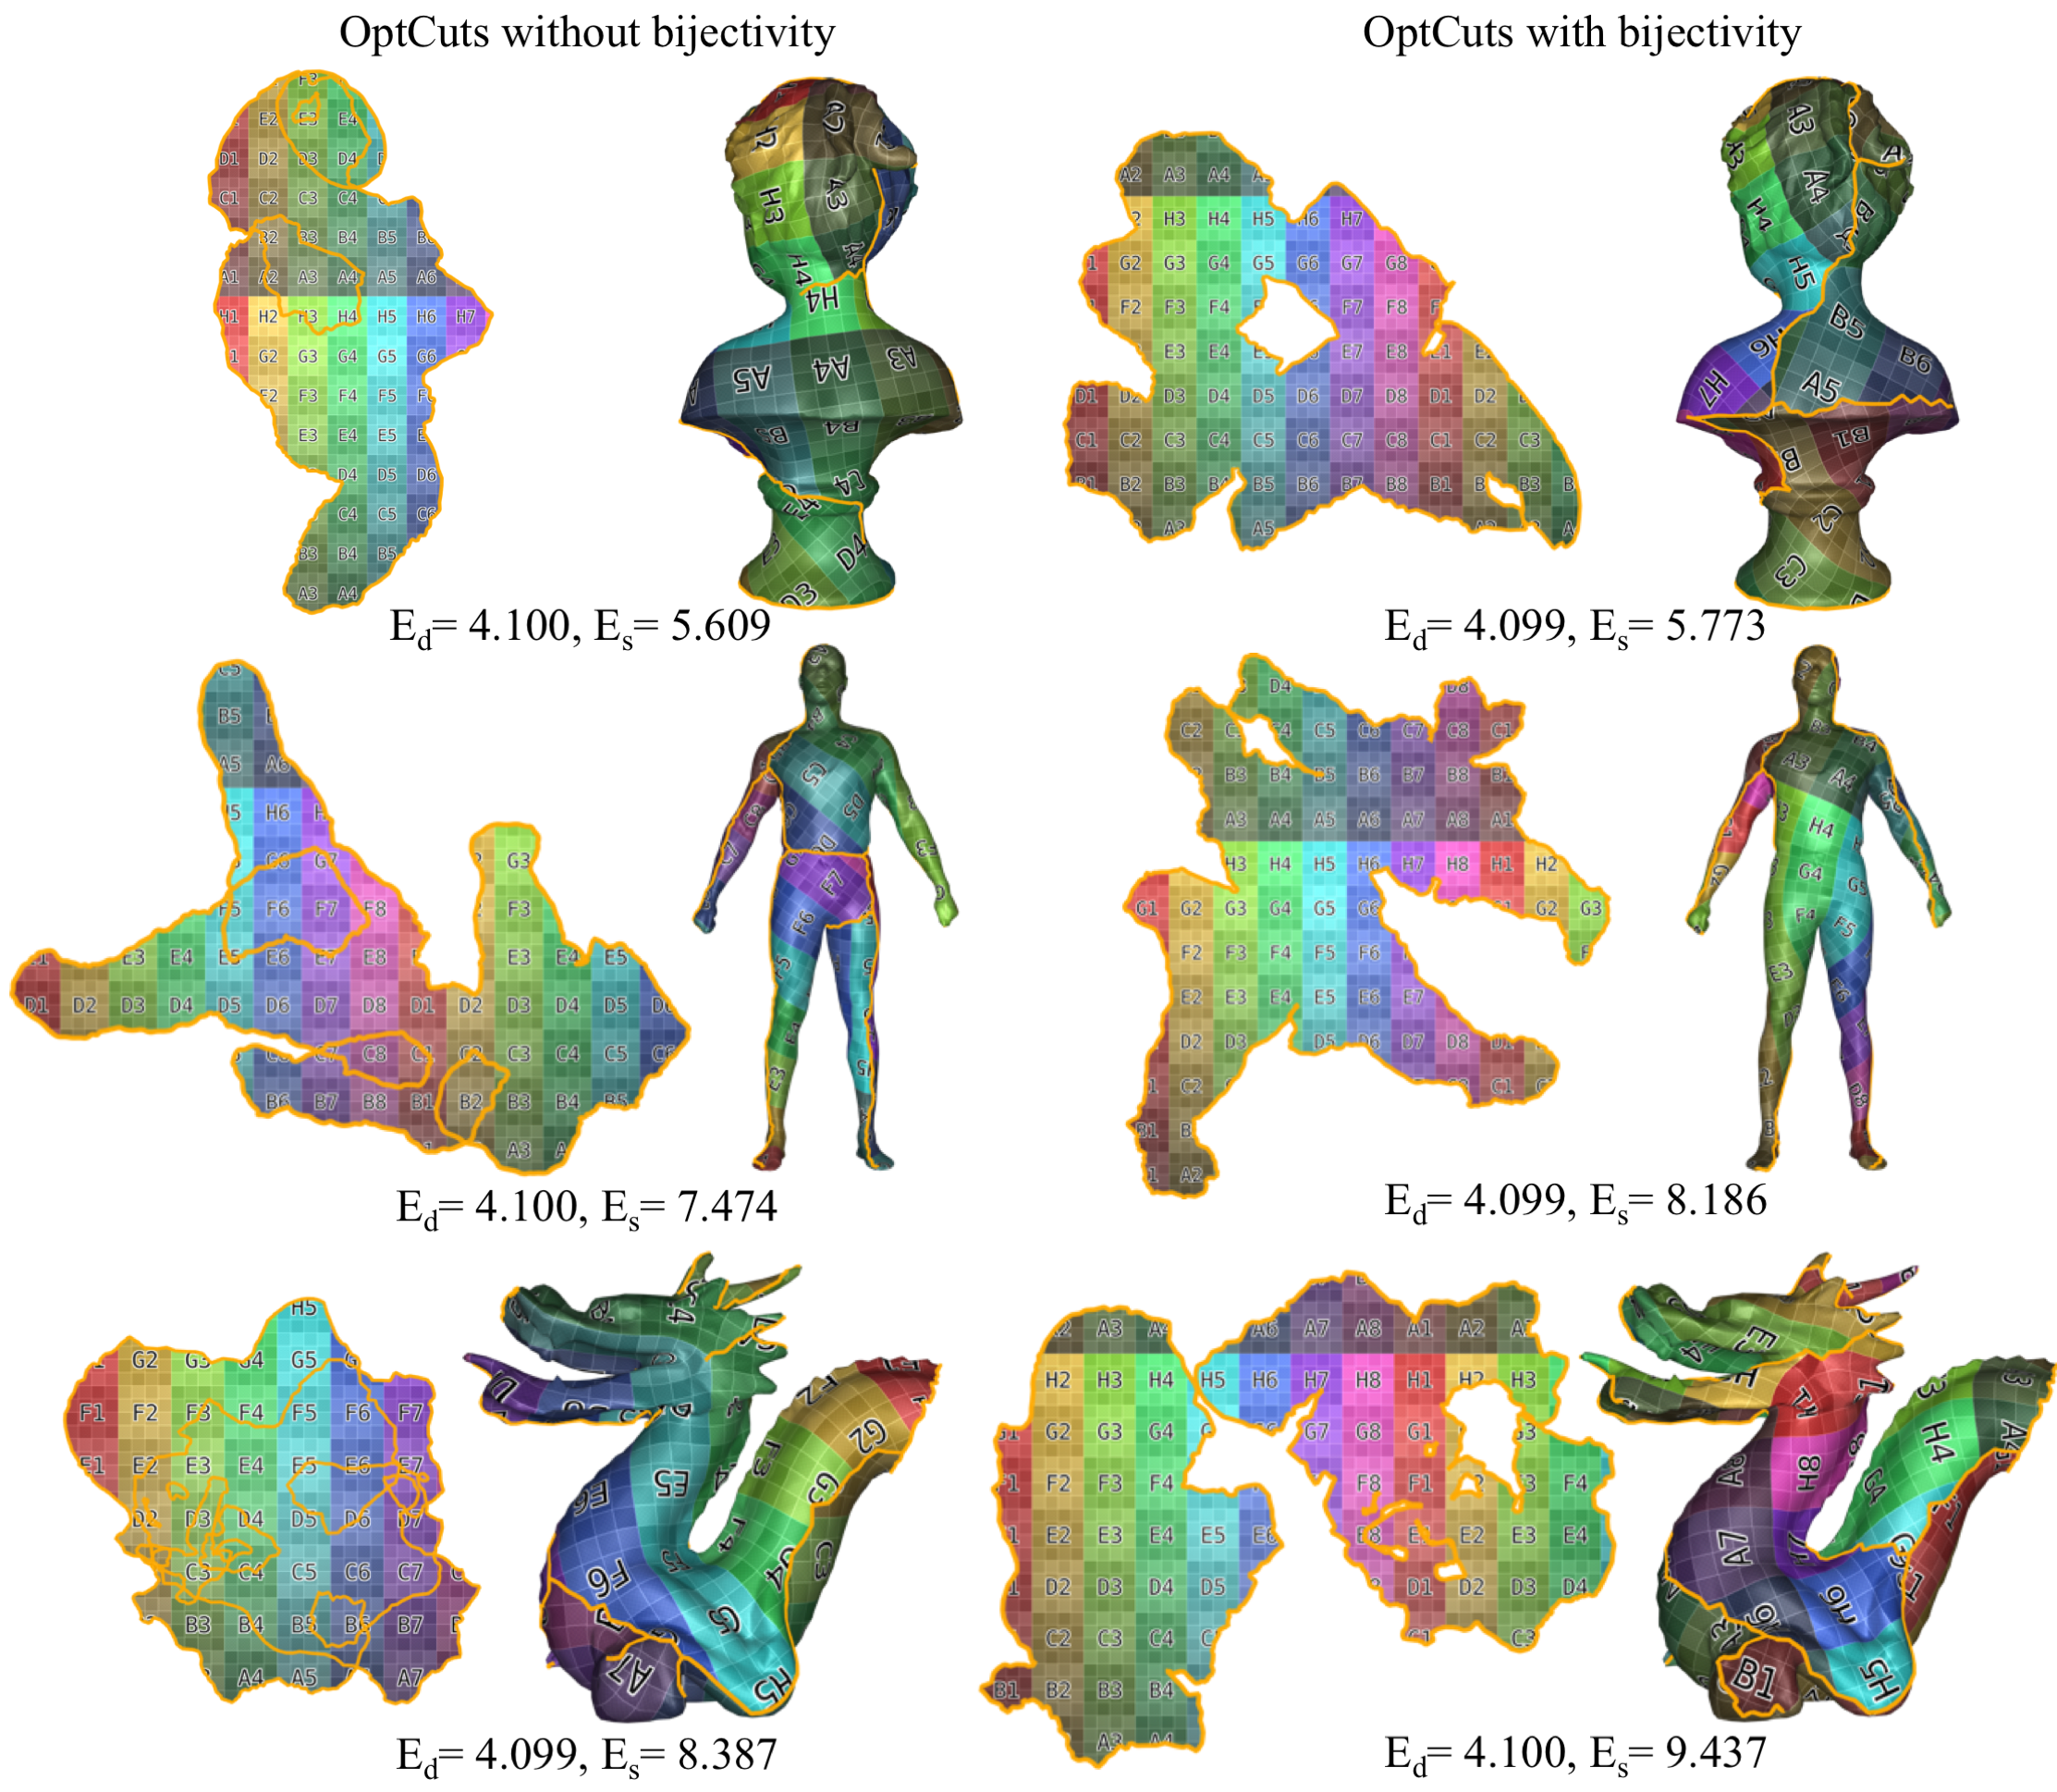
\includegraphics[width=\linewidth]{fig/our_impressive_results_right.png}
\caption{UV maps generated for various models by OptCuts with/without bijectivity with $b_d = 4.1$.}
\label{fig:our_impressive_results}
\end{figure}
%could also be bunny_i, statue_5, wooden_fish

\begin{table}[t]
\centering
\caption{OptCut performance on the benchmark of 70 surfaces with various distortion bounds. For each bound we try our method with and without global bijectivity.}
\label{tb:stats_OptCuts}
\begin{tabular}{|c|c|ccc|ccc|}
\hline
\multirow{2}{*}{$b_d$} & \multirow{2}{*}{bijectivity} & \multicolumn{3}{c|}{$E_{s}$} & \multicolumn{3}{c|}{time (s)} \\ \cline{3-8} 
                       &                         & avg      & min     & max      & avg       & min    & max      \\ \hline
\multirow{2}{*}{4.2}   & OFF                    & 3.819   & 0.080  & 14.545  & 87.0   & 0.3 & 417.8 \\
                       & ON                & 4.087   & 0.289  & 17.063  & 190.3   & 3.8 & 983.3  \\ \hline
\multirow{2}{*}{4.1}   & OFF                    & 4.709   & 0.752  & 17.980  & 137.5  & 0.9 & 886.9 \\
                       & ON                & 5.324   & 0.860  & 21.595  & 271.1   & 6.9 & 1767.8  \\ \hline
\multirow{2}{*}{4.05}  & OFF                    & 6.142   & 0.277  & 21.566  & 213.2  & 3.9 & 1398.1   \\
                       & ON                & 7.195   & 0.932  & 29.596  & 412.9   & 7.2 & 2859.5 \\ \hline
\end{tabular}
\end{table}

\subsection{Comparison to AutoCuts}
We compare our method to AutoCuts~\cite{Poranne2017Autocuts}, the state-of-the-art tool that jointly considers cutting and parameterization. 
They optimize a sum of seam penalty (weighted by $\lambda$) and distortion measure. In their formulation, the topology of the mesh does not change
(it is always a triangle soup), but seam penalty is parameterized by $\delta$ parameter which indicates how far the vertices have to be from one another
in order for them to be considered disconnected by a seam. Finding a single weight $\lambda$ that fits all geometries poses a challenge, and parameter
$\delta$ needs to be adjusted over time depending on the current stage of optimization. Thus, their method is the most effective with the user in the loop. For instance, starting with a disconnected triangle soup, the user gradually decreases $\delta$ defining a {\em homotopy path} over the course of optimization to arrive at a final set of seams. The user also needs to move parameterized components to guide the UV layout towards globally bijective solution. 
%
\vova{take a close look at the description above to make sure there are no mistakes. especially on user controls.}

%
We used publicly available implementation of AutoCuts and authors guidance us to devise a fully automatic version of their method that performed well on our benchmark.  The main challenge lies in constructing appropriate homotopy paths (i.e., the sequence of updates to $\delta$) with a uniform set of mesh-adaptive parameters. In this experiment, we set $\lambda = 0.4$ and started with $\delta_0=100\overline{|e|}^2$, and half it in the beginning of each homotopy iteration $\delta_i = \frac{1}{2}\delta_{i-1}$ until it reaches $\delta_\text{term}=10^{-4}\overline{|e|}^2$. Inside each homotopy iteration, we detect convergence by setting a tolerance $\sqrt{3n_t}\times10^{-3}\overline{|e|}$ on the $L^2$ norm of UV coordinate changes. Here $\overline{|e|}$ is the average edge length, $n_t$ is the number of triangles.
%
\vova{using the integer here seems a bit weird... can we explain this choice a bit more?}
\minchen{This makes the tolerance more invariant to mesh resolution. Imagine two meshes with same $\overline{|e|}$ but $100$ vertices and $100M$ vertices respectively...}

%
%AutoCuts obtains high quality UV maps by involving users into the optimization loop. However, when aiming for convenient, fully-automatic methods, the non-smoothness of their Separation energy not only makes it challenging for global parameter settings, but also often end up the optimization with suboptimal results. To show that we automatically generate high quality UV maps without suffering from these issues, we compare our method with a fully automatic version of AutoCuts obtained under the guidance of AutoCuts authors by constructing appropriate homotopy paths with a uniform set of mesh-adaptive parameters. 
%Specifically, we used $\lambda = 0.4$ and started with $\delta=100\overline{|e|}^2$ and half it in the beginning of each homotopy iteration until it reaches $10^{-4}\overline{|e|}^2$. Inside each homotopy iteration, we detect convergence by setting a tolerance $\sqrt{3n_t}\times10^{-3}\overline{|e|}$ on the $L^2$ norm of UV coordinate changes. Here $\overline{|e|}$ is the average edge length, $n_t$ is the number of triangles.

AutoCuts enables the user to control distortion indirectly by adjusting $\lambda$ parameter, but does not guarantee reaching a particular bound. Thus, to make our comparisons fully automatic we first run AutoCuts on an input surface, and then set the distortion measure for the AutoCuts output as the target bound $b_d$ for our method. Since automatic version of AutoCuts does not naturally support global bijectivity the most direct comparison is to the non-bijective version of our method, however, we compare to both variants for completeness.  As demonstrated in Table~\ref{tb:comp_AutoCuts} both versions of our method require less time to generate UV maps with significantly shorter seams while reaching the same level of distortion. Figure~\ref{fig:ESLBar_compAutoCuts} provides a more detailed comparison for every model in the benchmark, the bar charts are sorted by total seam length, where method with longer bars resulted in higher seams.
\vova{Minchen, would be good to say a few words about 2 shapes where our method produces slightly longer seams.} 
\minchen{It's the kingkong (10002 vertices) and cathead (131 vertices). For kingkong we only need 393.6s and 850.7s without/with bijectivity, but AutoCuts needs 1858s.}
%
%Note that we easily enforced bijectivity (Figure~\ref{fig:comp_AutoCuts}), which is only supported in AutoCuts with user assistance on patch manipulation.
%Since AutoCuts does not intuitively support generating UV maps with a certain level of distortion, we first run AutoCuts on a batch of input surfaces, and then set their output distortions as $b_d$ in our method for each input. As demonstrated in Table~\ref{tb:comp_AutoCuts}, for both the two versions of our method, we require less time to generate UV maps with same level of distortion but significantly smaller seams. Figure~\ref{fig:ESLBar_compAutoCuts} shows a bar chart comparison on the output $E_{s}$ of each input surface. Note that we easily enforced bijectivity (Figure~\ref{fig:comp_AutoCuts}), which is only supported in AutoCuts with user assistance on patch manipulation.

\begin{table}[t]
\centering
\caption{Comparisons between AutoCuts and OptCuts with/without bijectivity on all input surfaces in our dataset. We use AutoCuts output distortion (range from $4.016$ to $4.187$) as $b_d$ in our method for each input. Even with global bijectivity constraints our method achieves shorter seam lengths with shorter running times.}
\label{tb:comp_AutoCuts}
% \begin{tabular}{|c|ccc|ccc|}
% \hline
% \multirow{2}{*}{method} & \multicolumn{3}{c|}{$E_{s}$} & \multicolumn{3}{c|}{time (s)} \\ \cline{2-7} 
%                         & avg      & min     & max      & avg      & min    & max       \\ \hline
% AutoCuts                & 7.5789   & 1.2069  & 24.6816  & 499.9    & 4.0    & 2677.0    \\
% OptCuts(B)               & 5.8114   & 0.8979  & 19.7405  & 304.0    & 6.4    & 1267.7     \\
% OptCuts               & 5.3065   & 0.8992  & 16.1329  & 148.7    & 3.1    & 650.9    \\ \hline
% \end{tabular}
\begin{tabular}{|c|c|c|c|c|}
\hline
method                   & bijectivity & avg. $E_{d}$ & avg. $E_{s}$ & avg. time (s) \\ \hline
AutoCuts                 & N/A         & 4.074        & 7.5789       & 499.9         \\ \hline
\multirow{2}{*}{OptCuts} & ON          & 4.073        & 5.8114       & 304.0         \\
                         & OFF         & 4.073        & 5.3065       & 148.7         \\ \hline
\end{tabular}
\end{table}

\begin{figure}[t]
\centering
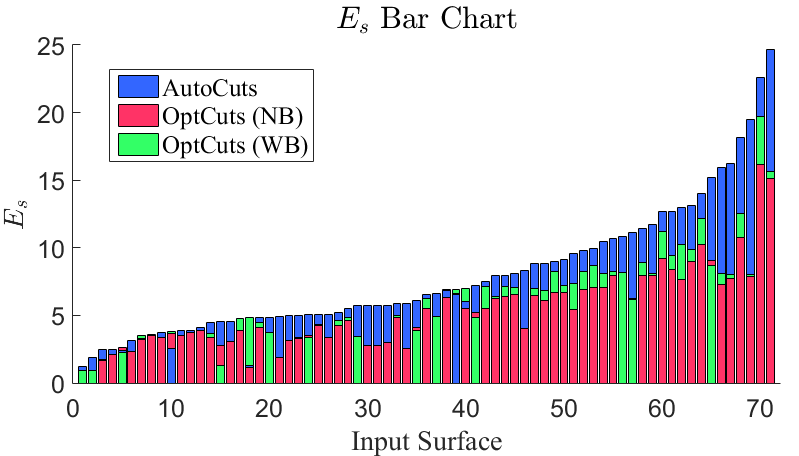
\includegraphics[width=\linewidth]{fig/ESLBar_compAutoCuts.png}
\caption{Normalized seam length $E_{s}$ bar chart of each example generated by AutoCuts and OptCuts. We (red) achieve shorter seams than AutoCuts (blue) for all except for two inputs, while reaching the same levels of distortion. Our method still performs favorably even with global bijectivity constraints (green).}
\label{fig:ESLBar_compAutoCuts}
\end{figure}

\begin{figure}[t]
\centering
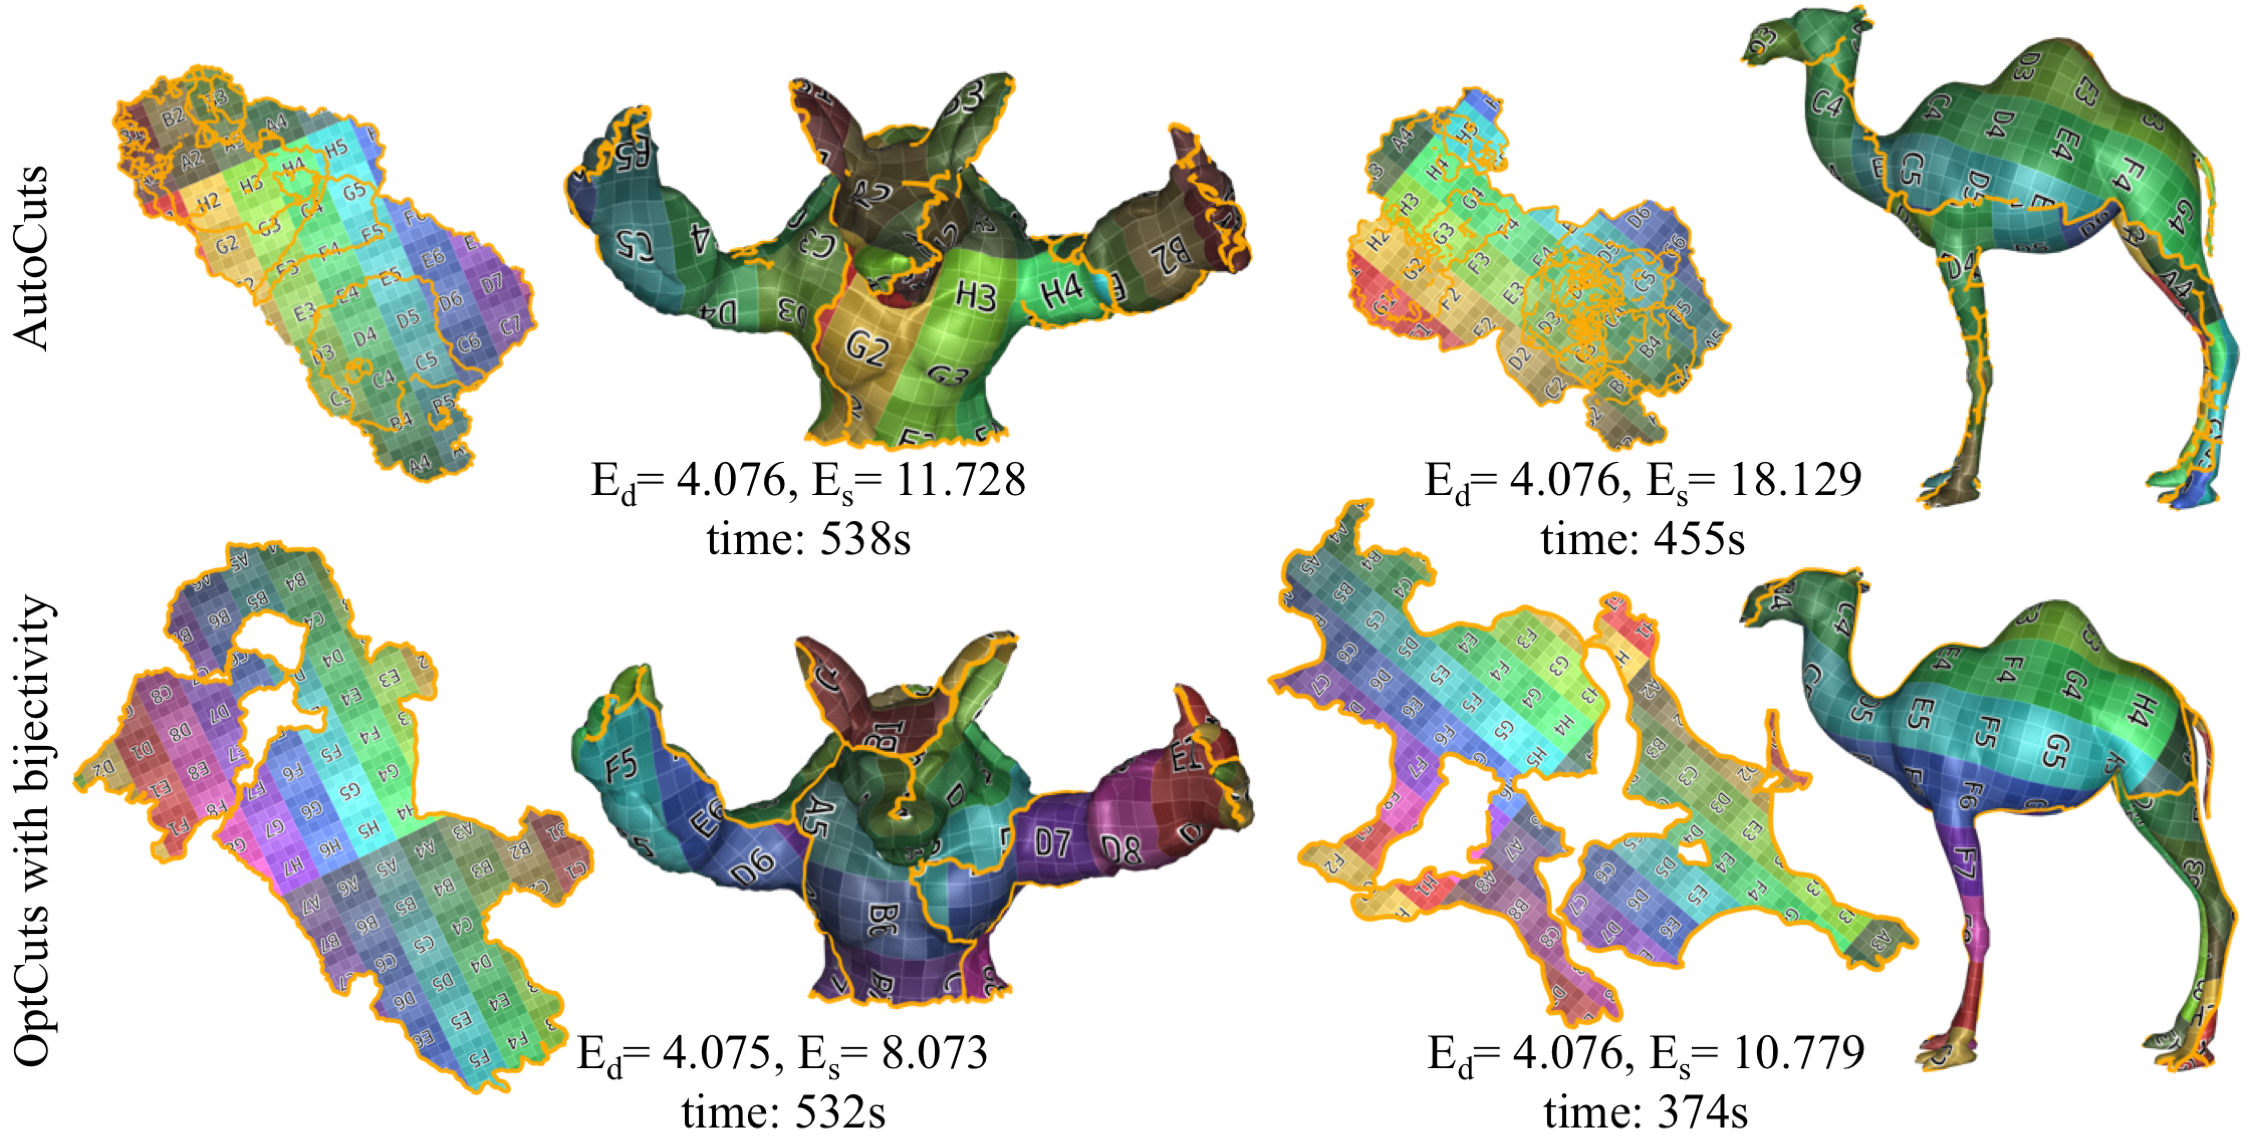
\includegraphics[width=\linewidth]{fig/comp_AutoCuts.png}
\caption{Comparison between AutoCuts (top) and OptCuts with bijectivity (bottom) on the armadillo (left) and camel (right) model. In this experiment the distortion bound was set to the same value as AutoCuts output, and our method achieved the bound with shorter seams. }
\label{fig:comp_AutoCuts}
\end{figure}
% could also be bone_noInput, bunny_i_f10000, bunny, camel_vova_f10000, cat_noUV, cow_param_closed, dilo, horse, male_2, octopus, wooden_fish, foot_i_f10000, three_man_statue, gargoyle, rgb_dragon, statue_i_1, vase, venus

\paragraph{Scalability}
We compare scalability of both methods by analyzing how the vertex count affects the running time. 
We present this as scatter plot over the benchmark meshes (Figure~\ref{fig:time_res_compAutoCuts}a), 
and test on a high resolution model of Lucy with 5 different levels of details (Figure~\ref{fig:time_res_compAutoCuts}b). 
For higher resolution models (24200 and 48354 vertices) AutoCuts ran out of memory, since their system is $x6$ times 
larger than ours. For the other models we see that gap between two approaches increases. Since our method 
adaptively updates topology of the mesh, we optimize with respect to a smaller number of variables that contributes
to substantial speedup (since only the vertices along the seam need to be duplicated). 
%
\vova{Danny -- I think you had a few other good points about scalability}
\minchen{e.g. data points not enough for fitting a trend; for input with 24200 vertices, system size of AutoCuts would be $24200 \times 2 \times 3 \times 2 = 290400$ v.s. $24200 * 2 = 48400$ of OptCuts; ...}

%From the time-resolution scatter plot in Figure~\ref{fig:time_res_compAutoCuts}a, we see that for meshes with higher resolution, our method scales better on running time than AutoCuts.
%We further run AutoCuts and our methods on 5 input surfaces obtained by progressively simplifying the original Lucy model (48354 vertices) to test scalability. From the trend in Figure~\ref{fig:time_res_compAutoCuts}b, we further see that our method scales better. Besides, the average $E_{s}$ obtained by our methods with/without bijectivity on the lucy models are $9.236$ and $8.816$ respectively, much smaller than $13.052$ by AutoCuts. Notice that for models with 24200 and 48354 vertices, AutoCuts already run out of memory, since its system size is $6$ times that of ours.

\begin{figure}[t]
\centering
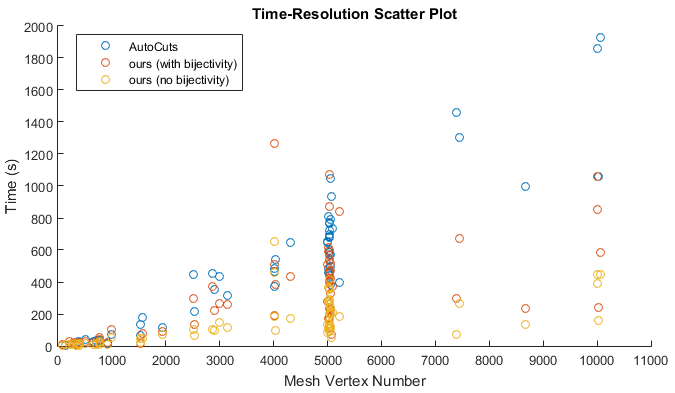
\includegraphics[width=\linewidth]{fig/time_res_compAutoCuts.png}
\caption{Time-resolution scatter plot of a batch of examples (a) and 5 lucy models with different resolutions (b) generated by AutoCuts (blue) and vanilla OptCuts (red) and with bijectivity enabled (green). In (b), there is no data points for AutoCuts on models with 24200 and 48354 vertices because they ran out of memory. Both versions of OptCuts require less computation on higher resolution meshes. OptCuts also achieve shorter average seams ($9.236$ with, and $8.816$  without bijectivity) than AutoCuts (13.052), while reaching same target distortion.}
\label{fig:time_res_compAutoCuts}
\end{figure}

\paragraph{Global Bijectivity}
\minchen{In AutoCuts paper, they mentioned in their Figure 11 that they experimented with a greedy procedure based on Sorkine et al.\ \shortcite{Sorkine2002Bounded} (Figure\ \ref{fig:comp_AutoCuts_Olga}a) to automatically handle bijectivity in AutoCuts (Figure\ \ref{fig:comp_AutoCuts_Olga}b). However, their result with user assisted patch manipulation still ends up with shorter seams (Figure\ \ref{fig:comp_AutoCuts_Olga}c). We execute OptCuts with bijectivity constraints on this example, setting the distortion of their user assisted output as $b_d$. We find that OptCuts achieves shorter seams with bijectivity automatically handled without the need of any user assistance (Figure\ \ref{fig:comp_AutoCuts_Olga}d).}

\begin{figure}[t]
\centering
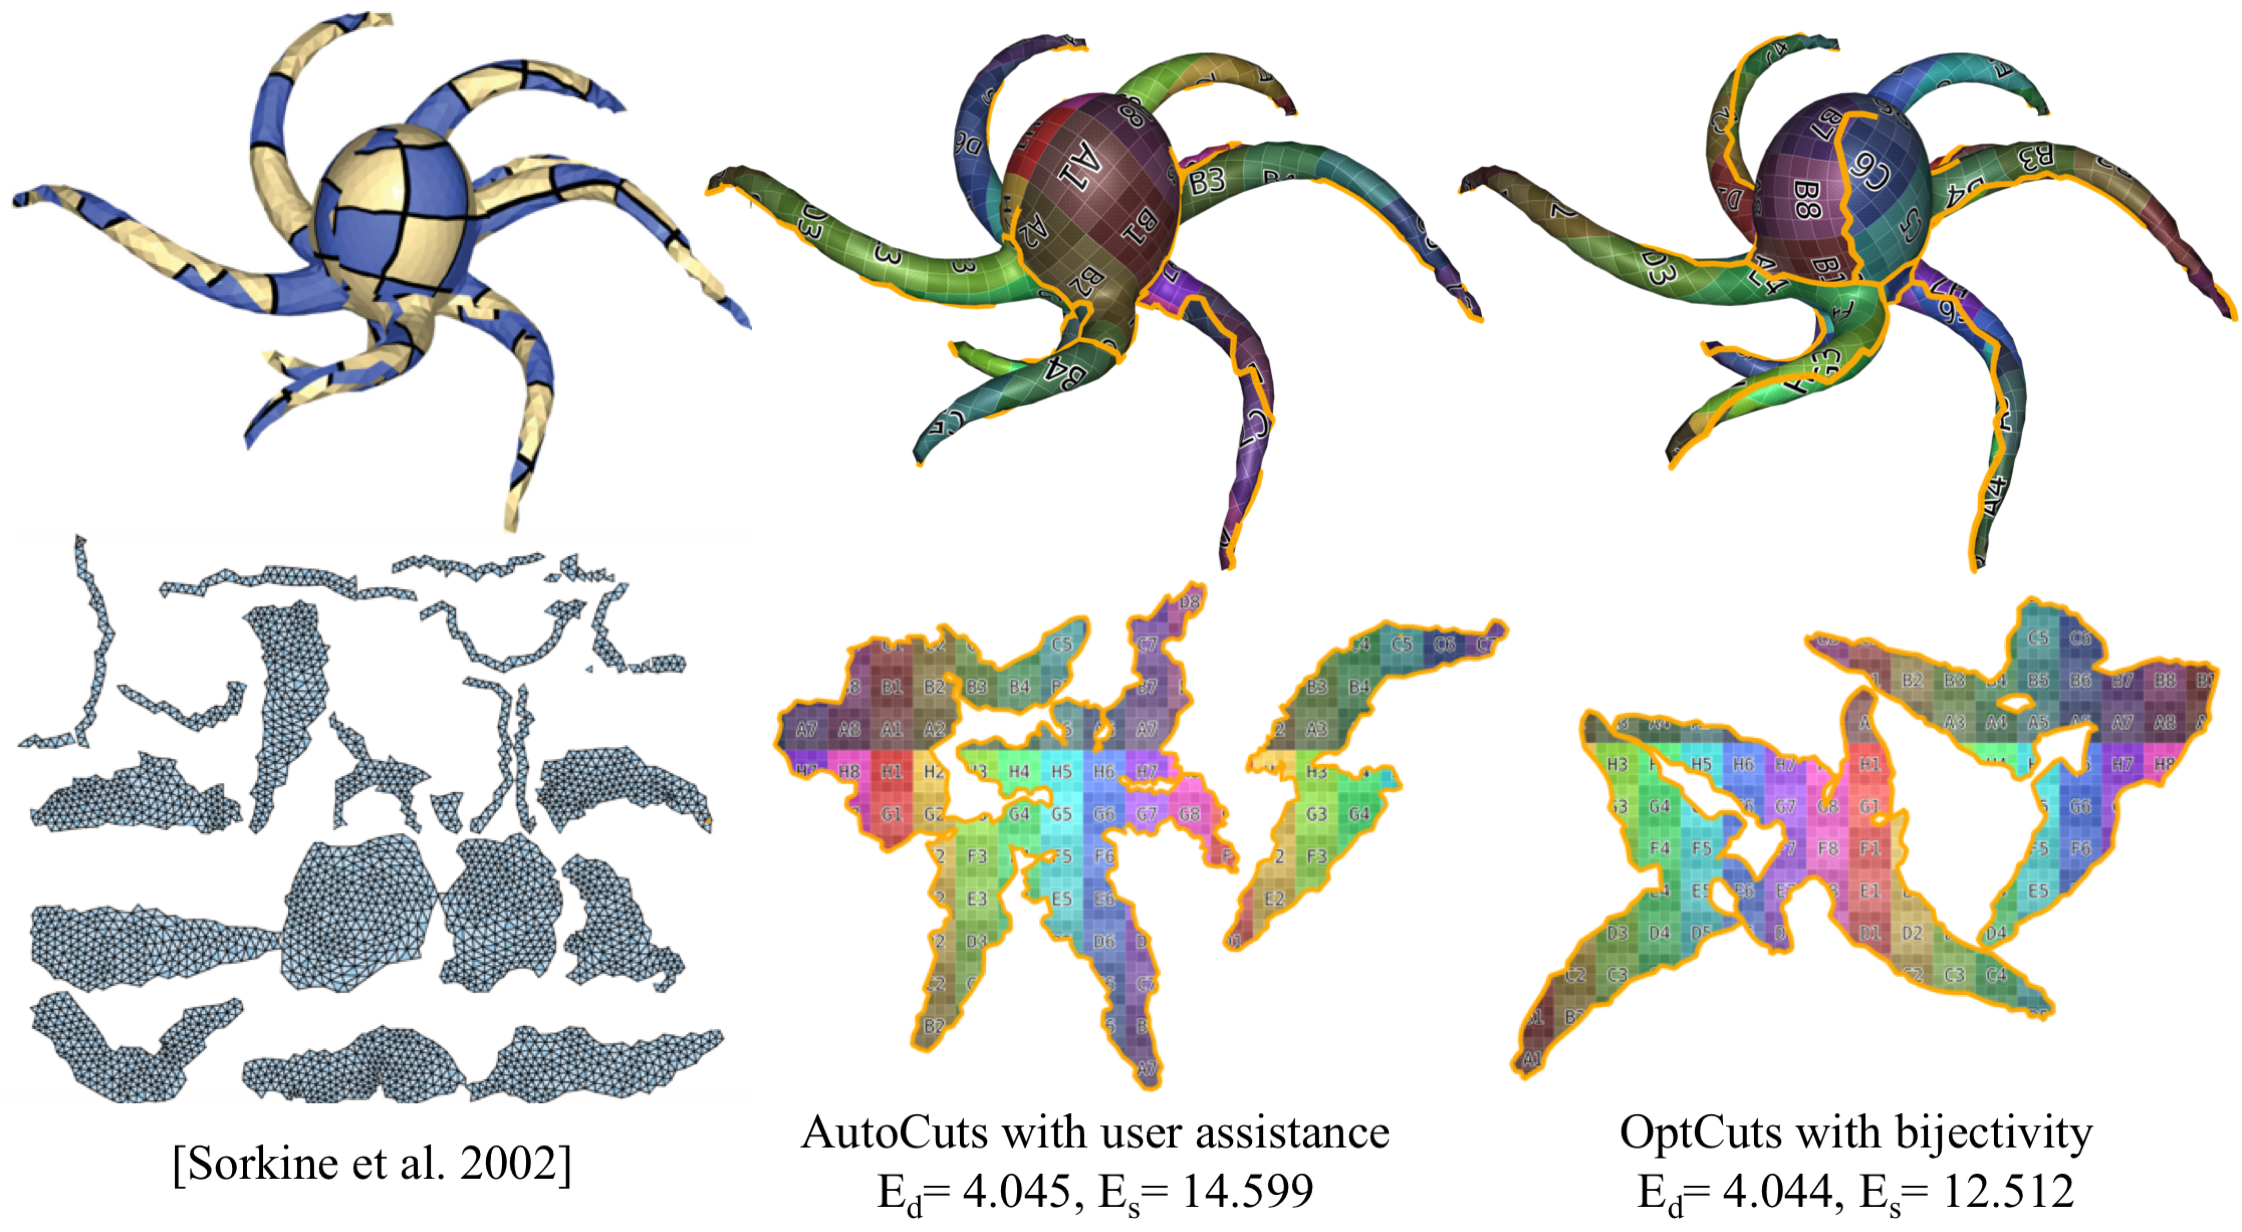
\includegraphics[width=\linewidth]{fig/comp_AutoCuts_Olga.png}
\caption{\minchen{I suggest we also add the result where AutoCuts tried to automatically handle global bijectivity}}
\label{fig:comp_AutoCuts_Olga}
\end{figure}


\subsection{Variations}

\paragraph{Regional Seam Placement}
Discontinuities produced by seams make texture assignment more challenging and might lead to unpleasant rendering artifacts. Thus, UV artists often guide seam placement away from the salient surface regions (e.g., human face). Our framework naturally enables the user to prevent placing cuts in some regions by painting over the surface, and we simply update the seam cost by assigning infinite weight in user-prescribed regions:
\[ \hat{E}_{s} = \sum_{i\in\mathcal{S}} w_{s,i} E_{s,i} \quad w_{s,i} \in [1.0, +\infty] \]

Figure~\ref{fig:regional_seam_placement} shows OptCut output without user guidance (top) and with the user-painted map of salient regions (blue function, middle), yielding a comparable seam length and distortion, but with better-placed seams (bottom). 
%
%In texture painting applications, users would really like regions with the same semantic meanings stay connected or close to each other on the UV map. If we let users to select those regions on the input surface, we could easily avoid seams in those regions while still achieving bijectivity and similar seam length under the same distortion bound (Figure~\ref{fig:regional_seam_placement}). Without changing our framework, we just need to modify our formulation of $E_s$ by weighting each seam edge using the indicator function $w_{s}$ provided by the user:


\begin{figure}[t]
\centering
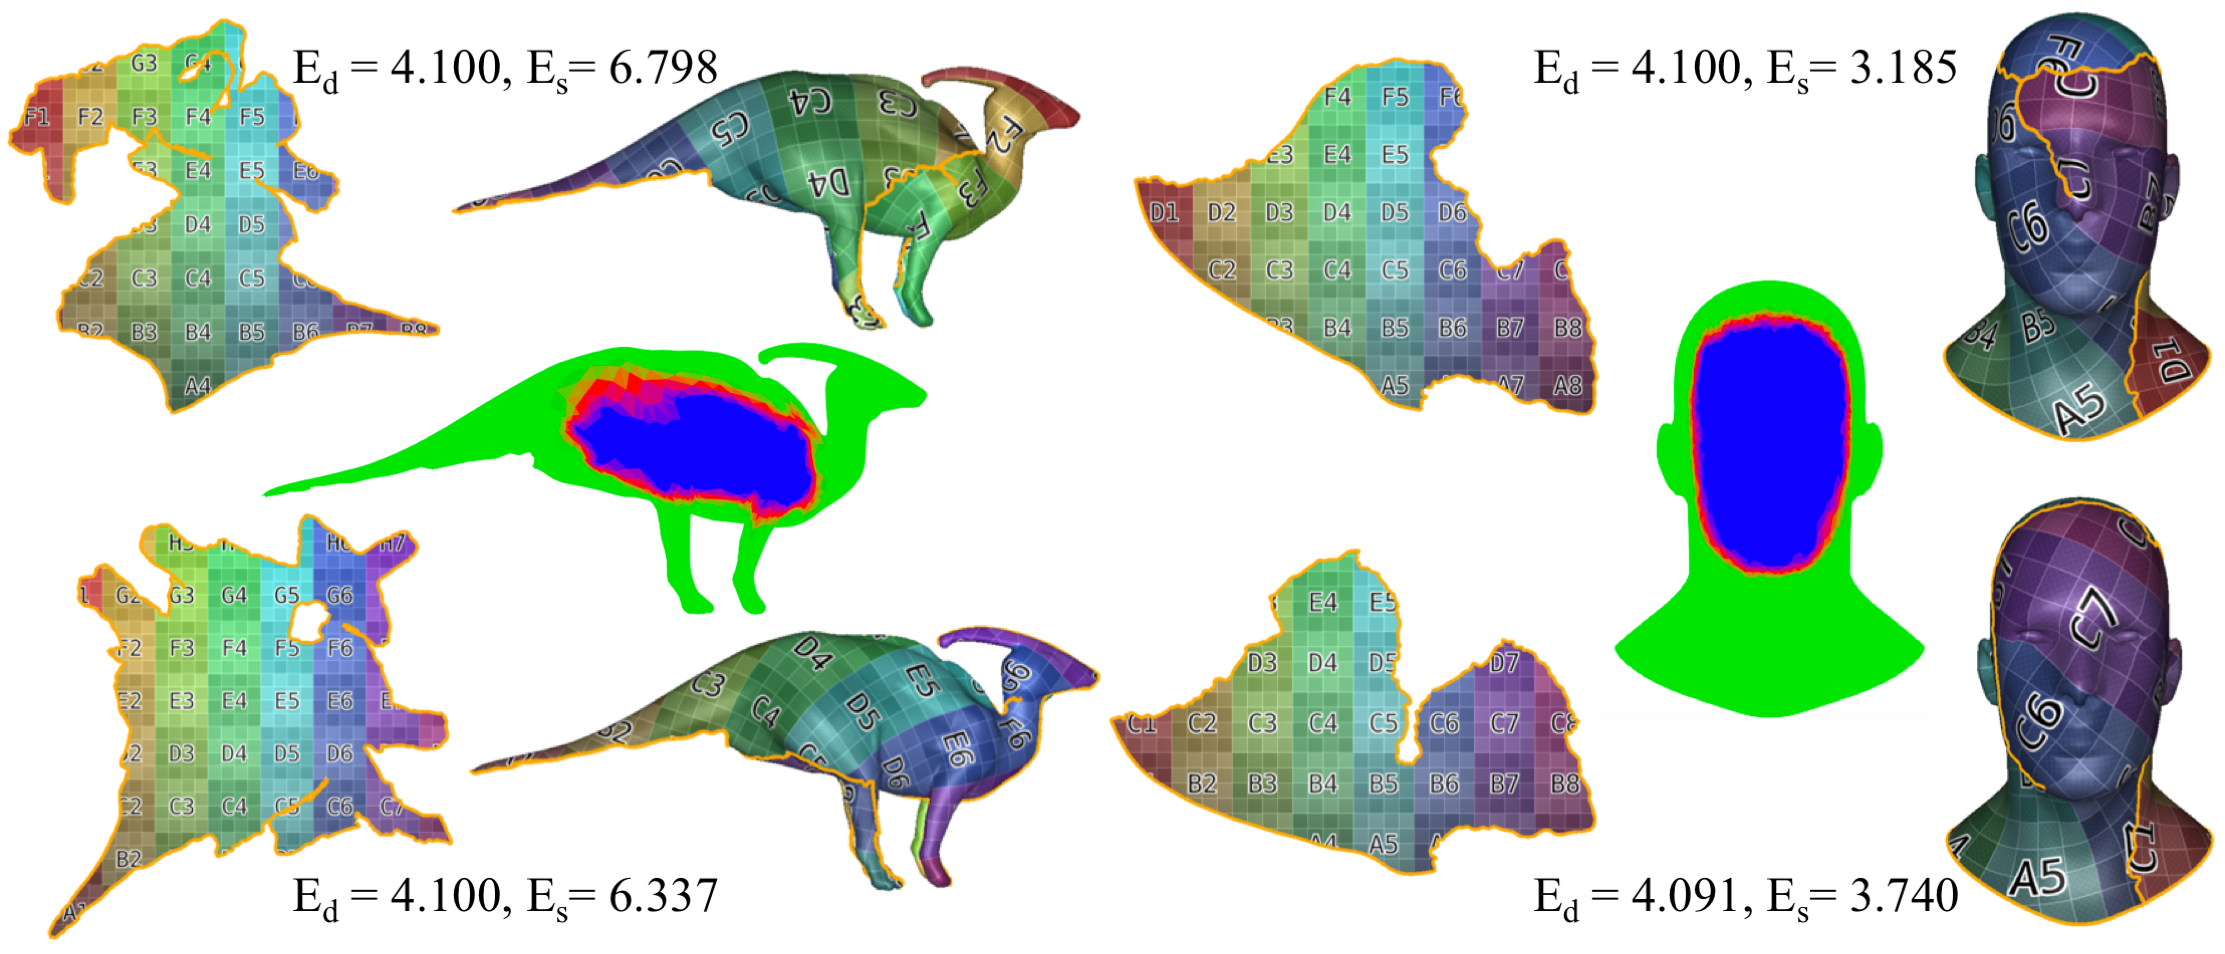
\includegraphics[width=\linewidth]{fig/regional_user.png}
\caption{Two examples with user-guided seam placement. The distortion bound is set to $b_d=4.1$ and we enforce bijectivity constraints in both cases. 
The fully automatic OptCut solution might place seams in salient regions (top), but the UV artist can paint ``do not cut here'' function (middle, blue), which will guide
the OptCut towards a better seam placement (bottom). Note that distortion and seam length is comparable in both cases. We happen to achieve shorter seams with additional user constraints for the dinosaur model since our method searches for a local optimum.}
\label{fig:regional_seam_placement}
\end{figure}

% \paragraph{Conformal Parameterization}
% Using a conformal energy~\cite{Hormann2000MIPS,Sheffer2005ABFPP} for $E_d$ will achieve joint seam placement and conformal parameterization. Figure~\ref{fig:conformal_vs_isometry} shows some results with $E_d = E_{ABForMIPS}$~\cite{} compared to results with $E_d = E_{d}$, where different seams are generated while our framework stays the same.

\paragraph{Alternative Cutting Strategy}
Our topology descent step leverages a small set of local topological operations to keep the framework simple and general. We also reduce the search complexity by filtering the candidates. Alternatively, one can use a richer set of more aggressive topological operations. For example, Geometry Images~\cite{Gu2002Geometry} leverage extrema-to-boundary cuts that connect the current boundary to the most distorted point (under current parameterization) using the shortest geodesic path. The advantage of this strategy is that it introduces more drastic topological updates at each iteration, potentially saving computational effort. We replace our topological search with this strategy (still terminating once $b_d$ is reached) and refer to the resulting variant of our method as EBCuts. As expected we found that the resulting approach is faster, however, we found that it yields longer seams, especially with tighter distortion bounds (Table~\ref{tb:comp_GI}), and for nearly isometric UV maps where extremities are less prominent (Figure~\ref{fig:comp_GI}).

\vova{We used notation $\mathcal{G}_T$ here, I don't think it appeared anywhere in the paper, so I removed it... we can define it earlier and bring it back if necessary...}

%The cutting strategy in the topology descent steps essentially build up the structure of the UV topology graph $\mathcal{G}_T$. By considering local topological operations, we built a dense graph connecting almost all the possible UV topologies and then reduce the search complexity by filtering. Alternatively, one can consider building $\mathcal{G}_T$ using only a sparse set of UV topologies and more aggressive topological operations, like the extremity-boundary (EBCuts) cut applied in Geometry Images~\cite{Gu2002Geometry}.


%We could alternatively apply EBCuts strategy in our framework without bijectivity constraints by simply alternating the cut with distortion minimization processes, and stop right after $b_d$ is reached. This variation of our method reaches identical distortion bounds with very similar seam length compared to our standard method, but is much faster since the EBCuts cut can be decided nearly instantly (Table~\ref{tb:comp_GI}). However, when we set smaller distortion bounds, the quality of the seams by EBCuts cut drops since extremities are not that obvious on a nearly isometric UV map (Figure~\ref{fig:comp_GI}).

\begin{table}[t]
\centering
\caption{Comparison between the standard OptCuts and using EBCuts cutting strategy in our framework, both without bijectivity constraints. We run the two methods on our benchmark and report statistics. EBCuts variant of our method is faster, but tends to produce longer seams.} 
\label{tb:comp_GI}
\begin{tabular}{|c|c|ccc|ccc|}
\hline
\multirow{2}{*}{$b_d$} & \multirow{2}{*}{strategy} & \multicolumn{3}{c|}{$E_{se}$} & \multicolumn{3}{c|}{time (s)} \\ \cline{3-8} 
                       &                         & avg      & min     & max      & avg       & min    & max      \\ \hline
\multirow{2}{*}{4.2}   & OptCuts                    & 3.819   & 0.080  & 14.545  & 87.0   & 0.3 & 417.8 \\
                       & EBCuts                & 3.868   & 0.159  & 14.929  & 13.0   & 0.1 & 72.1  \\ \hline
\multirow{2}{*}{4.1}   & OptCuts                    & 4.709   & 0.752  & 17.980  & 137.5  & 0.9 & 886.9 \\
                       & EBCuts                & 4.795   & 1.207  & 16.895  & 17.0   & 0.1 & 87.2  \\ \hline
\multirow{2}{*}{4.05}  & OptCuts                    & 6.142   & 0.277  & 21.566  & 213.2  & 3.9 & 1398.1   \\
                       & EBCuts                & 6.335   & 0.328  & 23.051  & 24.1   & 0.1 & 115.4 \\ \hline
\end{tabular}
\end{table}

\begin{figure}[t]
\centering
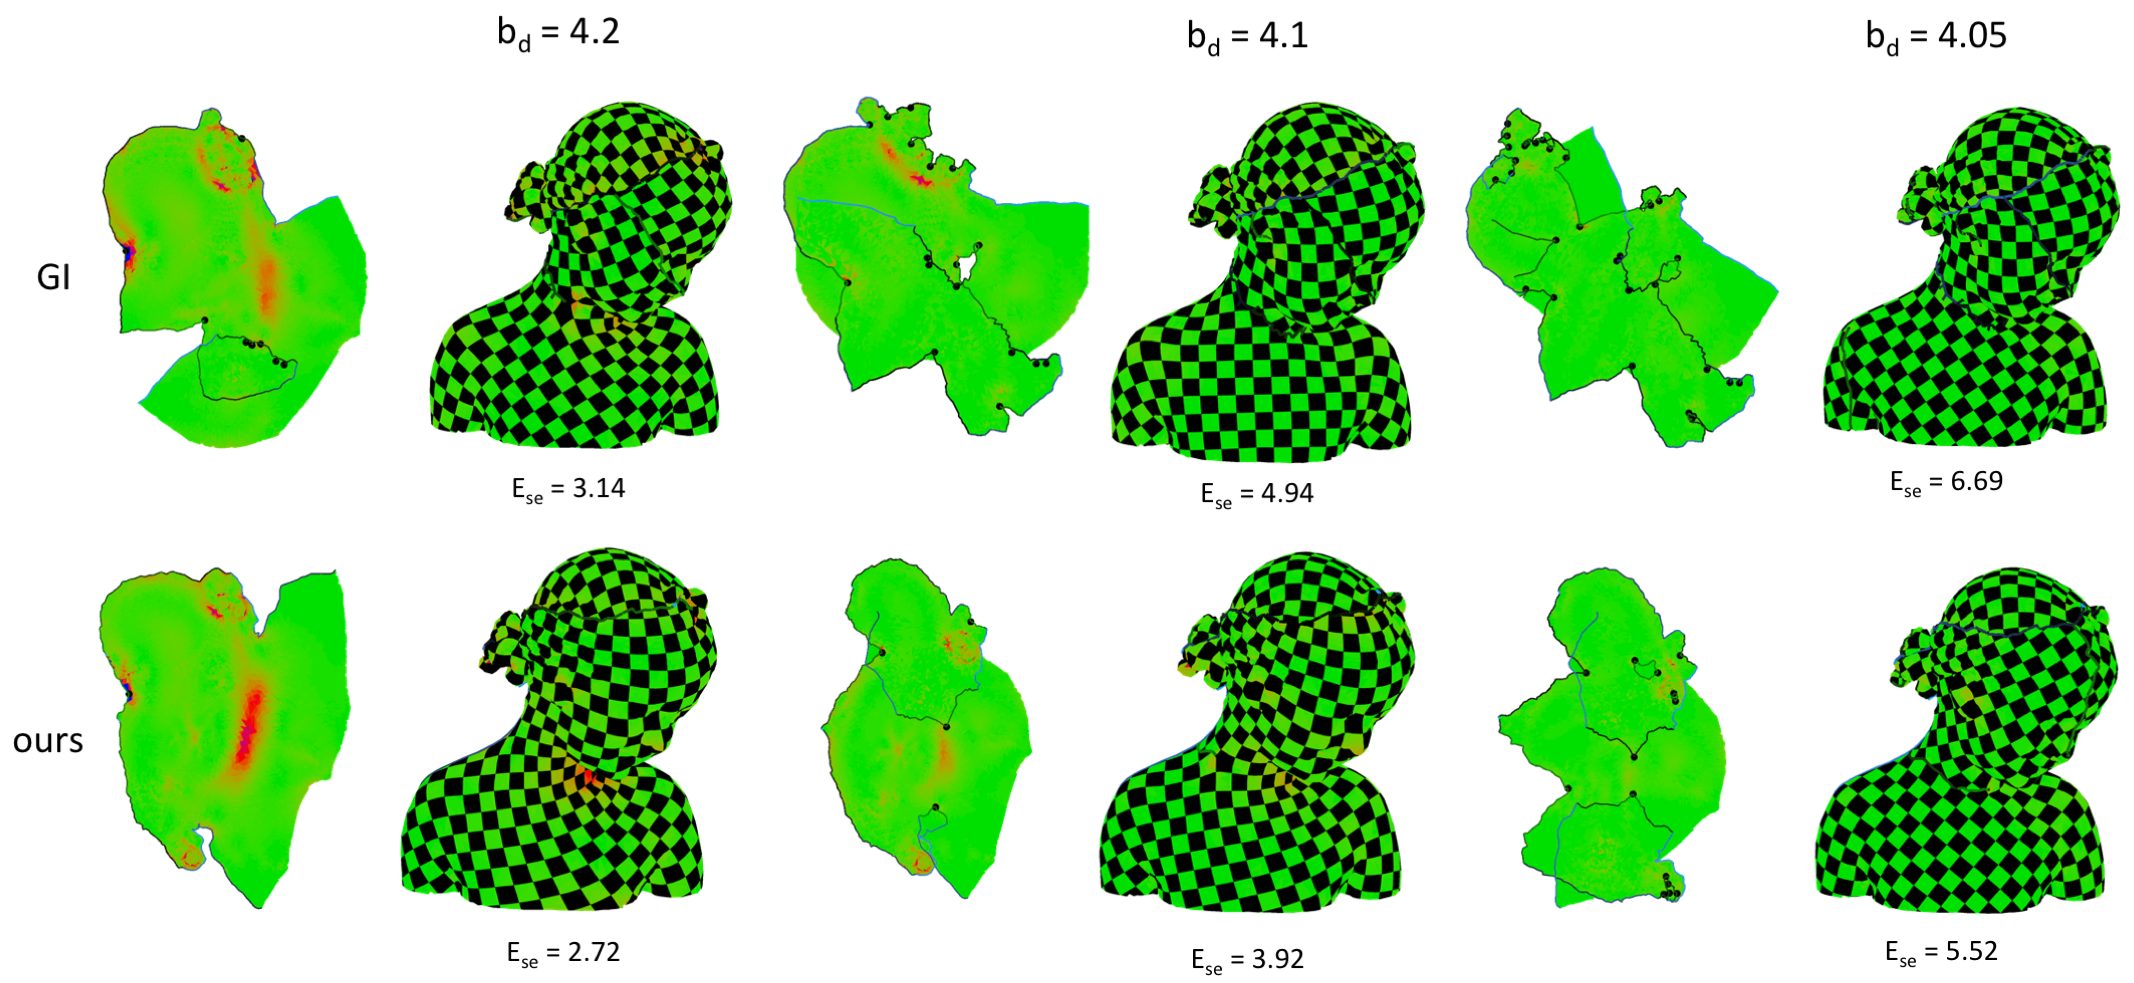
\includegraphics[width=0.8\linewidth]{fig/comp_GI.png}
\caption{Comparison between the standard OptCuts (left) and using EBCuts strategy in our framework (right), both without bijectivity constraints. EBCuts cutting strategy is very efficient in early stages (a, b), but it does not work well when the UV map gets closer to isometric where extremities are not very prominent (c).}
\label{fig:comp_GI}
\end{figure}
% also could be face_f10000, male_body_i_f10000, statue_4_i_f10000, statue_5_i_f10000, bimba_i_f10000

\paragraph{Warm Start}
Since our framework only provides a local optima for a highly non-convex problem, initial conditions are relevant for the final result and computational cost. Several powerful topological heuristics have been used to provide a disk-like topology for the geometry optimization algorithm. We can consider all of these methods as a way to define initial conditions for our approach. 

%Although we obtain high quality results given any initial embedding, the starting point does affect which local optimal point we will reach. Hence, it is meaningful to explore our method starting from initial seams with global observations. This will also benefit practical scenarios for improving preliminary UV maps while stay close to it.

As first example, we take the resulting seams produced by our method with EBCuts strategy and construct the initial embedding using our standard approach (Tutte's parameterization followed by distortion minimization). We can improve the seam quality while respecting the distortion bound by leveraging our local topological search which enables us to close up unnecessary cuts by merging. Even with the bijectivity constraints, we still achieve shorter seam length (Figure~\ref{fig:comp_GI_outputAsInit}).

\begin{figure}[t]
\centering
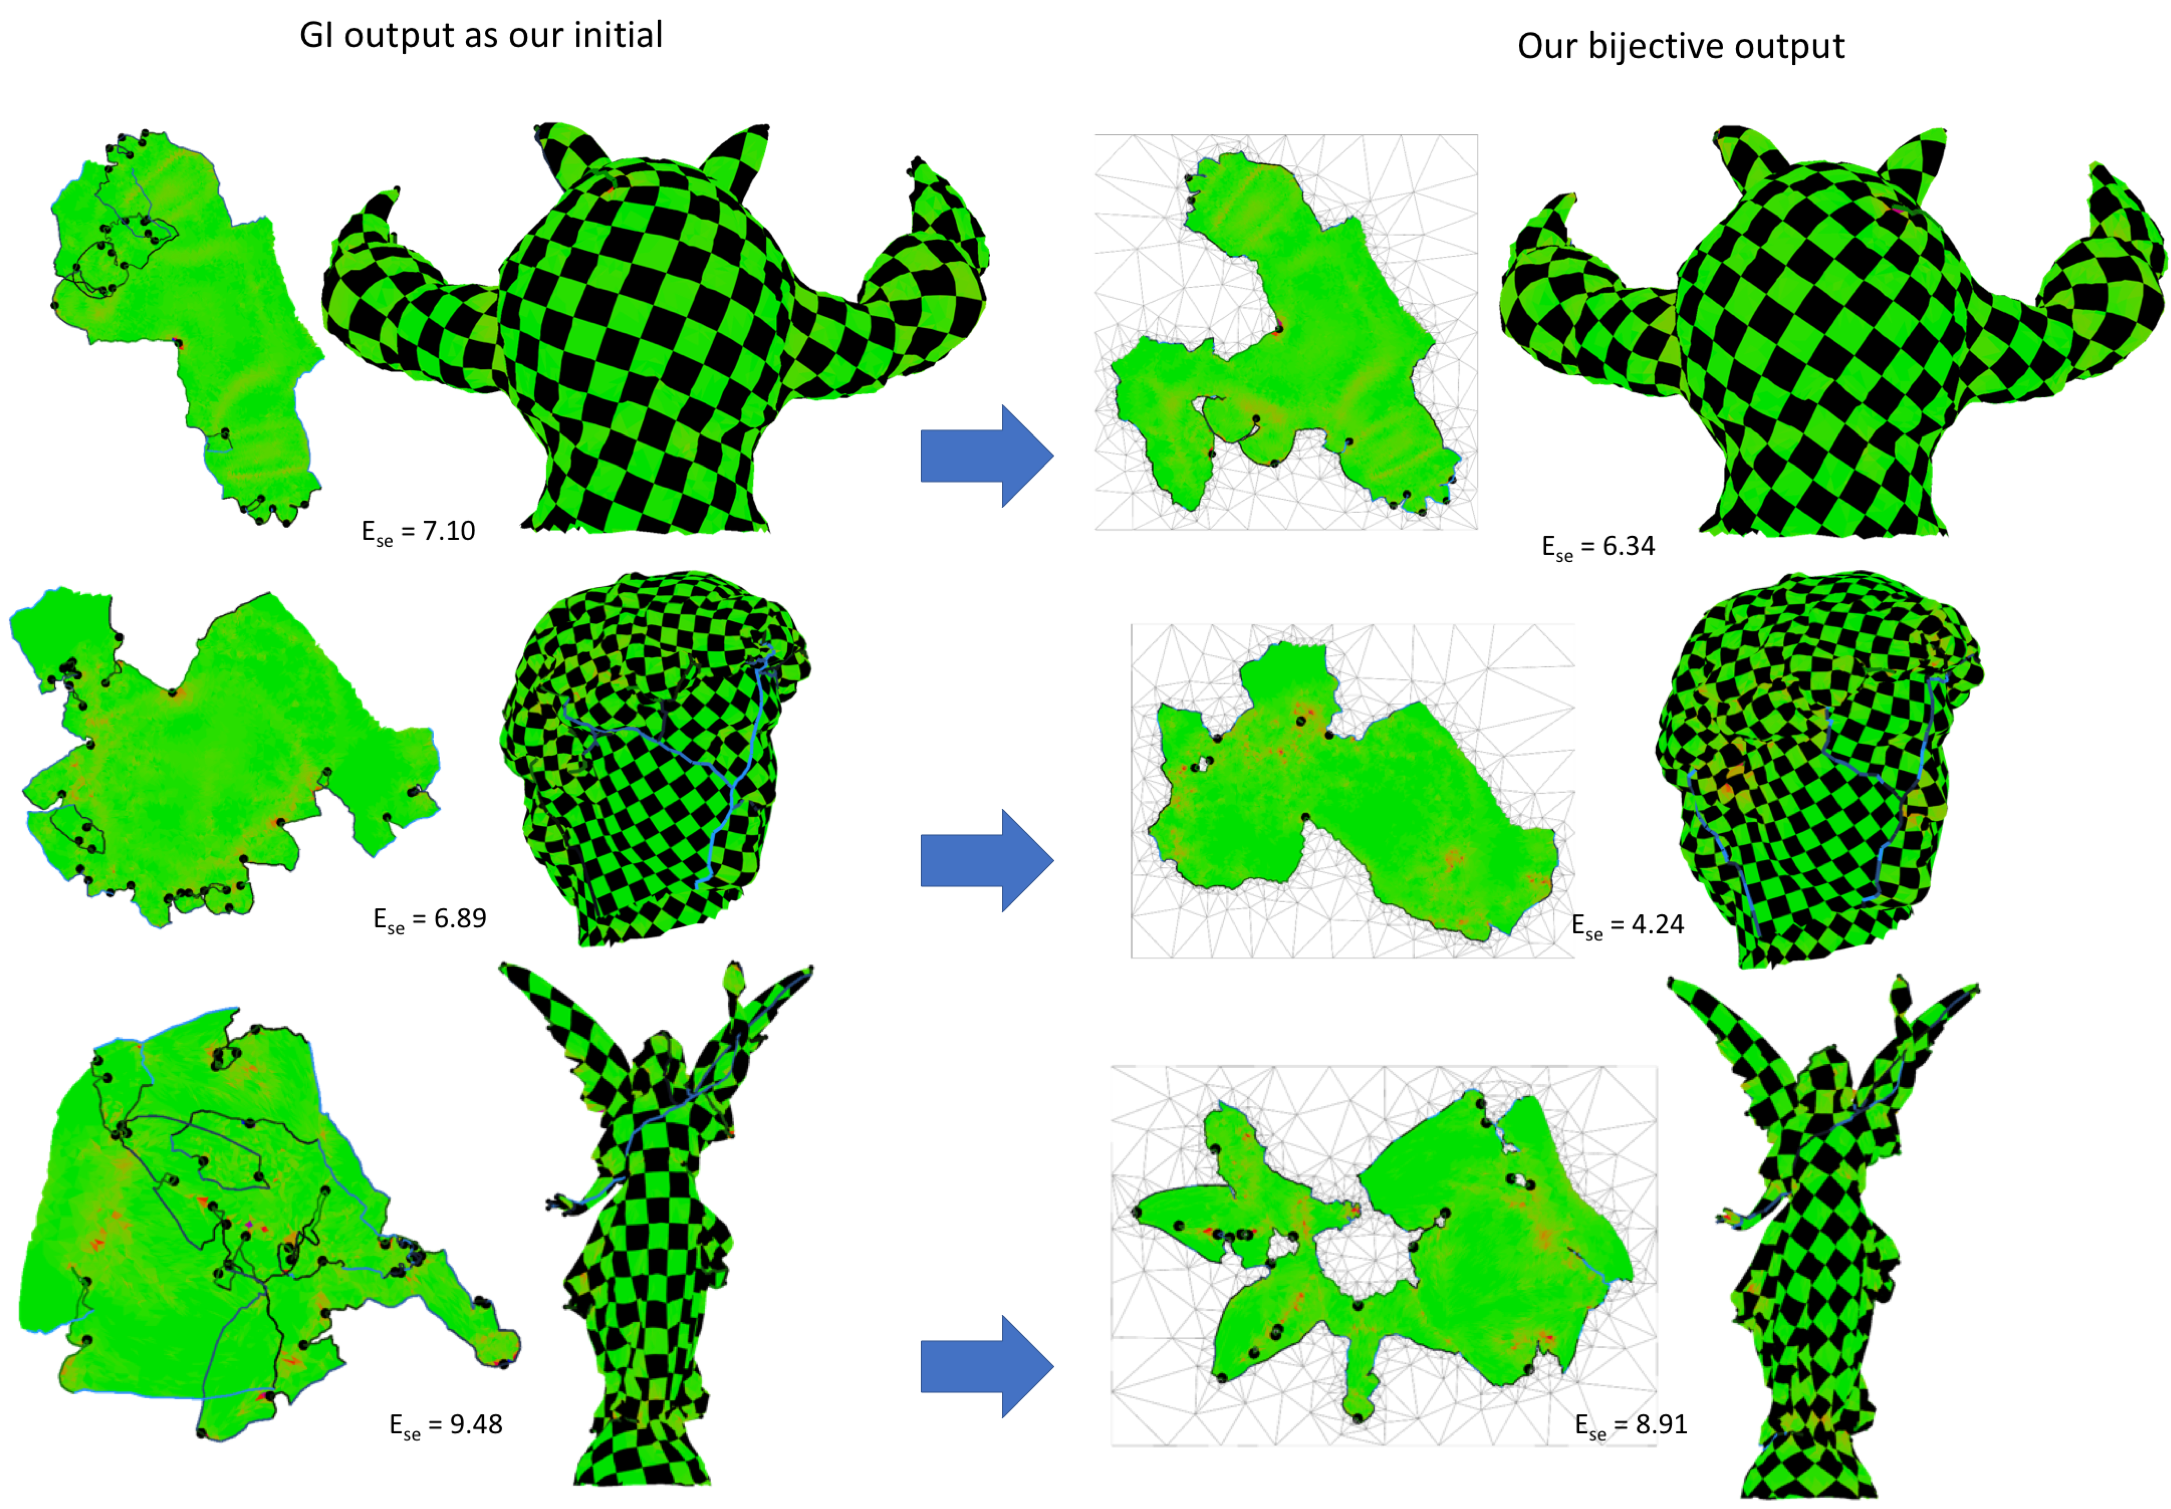
\includegraphics[width=\linewidth]{fig/comp_GI_outputAsInit.png}
\caption{We use the seams produced by our framework with EBCuts strategy at $b_d = 4.1$  initial UV map (a). We ran our OptCuts framework to improve the seam quality, reaching a locally optimal seam configuration under the given distortion bound even with bijectivity constraints (b). This seam length is also shorter than results obtained by standard OptCuts without bijectivity (c).}
\label{fig:comp_GI_outputAsInit}
\end{figure}
% also could be bimba, bunny

The second option we explore is Seamster~\cite{Sheffer2002Seamster}, a classic seam cutting strategy that detects local curvature extrema points and connects them with a minimal spanning tree.  This approach can be sensitive to the user-set parameters such as size of surface regions for computing local extrema, which is shape-dependent parameter that might require some user tuning. However, in this experiment we pick two models that have been successfully cut with Seamster (a cow and a triceratops), and use our standard approach to produce the initial embedding, i.e., Tutte's embedding followed by minimizing $E_{d}$ with bijectvitiy constraints (Figure~\ref{fig:comp_Seamster}a). We use the resulting distortion as the upper bound and run full OptCuts framework on the result. As demonstrated in Figure~\ref{fig:comp_Seamster}b, we achieve shorter seam length while maintaining the distortion bound and bijectivity. This seam length is also shorter than running our standard method without bijectivity from standard initialization (Figure~\ref{fig:comp_Seamster}c).

%With Seamster's best output seams on the cow and triceraptop model, we obtain UV maps by minimizing $E_{d}$ with bijectivity constraints (Figure~\ref{fig:comp_Seamster}a), and use them for warm start, setting their distortions as the upper bounds. As demonstrated in Figure~\ref{fig:comp_Seamster}b, we achieve shorter seam length while maintaining the distortion bound and bijectivity. This seam length is also shorter than running our standard method without bijectivity from standard initialization (Figure~\ref{fig:comp_Seamster}c).

\begin{figure}[t]
\centering
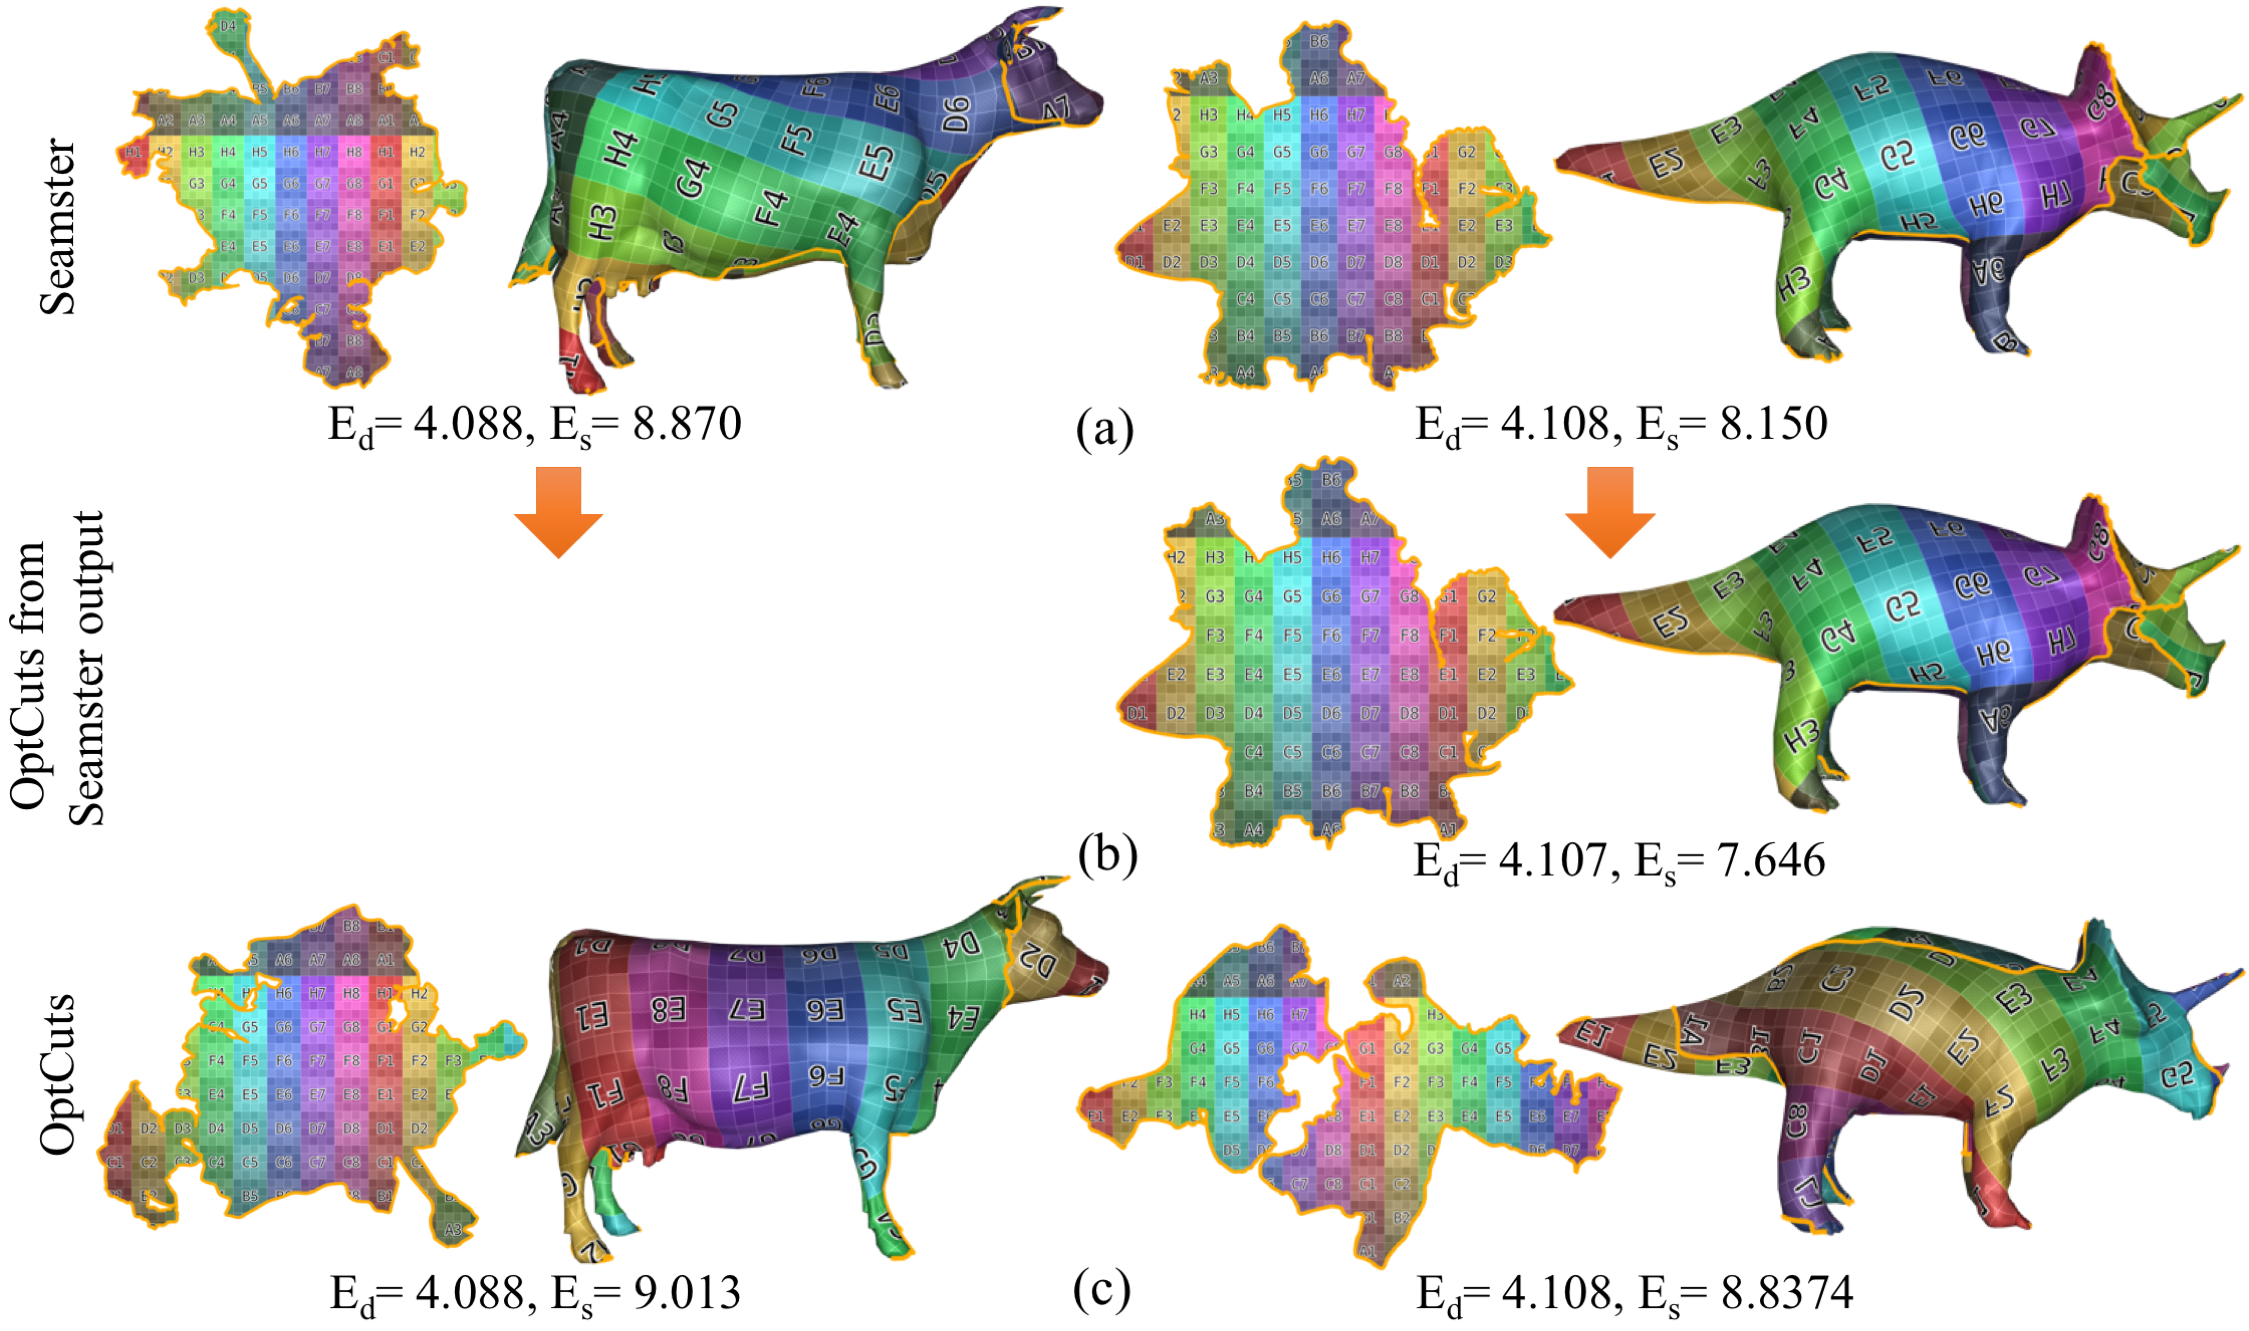
\includegraphics[width=\linewidth]{fig/comp_Seamster.png}
\caption{Starting from UV maps obtained by using Seamster's best output seams (a), we improve seam quality, reaching a locally optimal seam configuration while maintaining the distortion and bijectivity (b). This seam length is also shorter than running standard OptCuts without bijectivity from standard initialization (c).}
\label{fig:comp_Seamster}
\end{figure}

%For Seamster, user need to set the size of local regions for measuring extremity, which is a mesh and shape dependent parameter that requires fine tuning. Even OptCuts with standard initialization achieves similar seam length without any user assistance.

